% Williams Physics Thesis template
% Patterned after the work of Cole Meisenhelder '15
% Commented by Prof. Charlie Doret, 12/2016
% Uploaded to Overleaf by Dr. Kevin Flaherty, 5/2021

\documentclass[12pt, oneside]{book}

% The \usepackage{} command will import predefined fonts, symbols, environments, etc.  For example, the ams packages below come from the American Mathematical Society and include all kinds of useful math symbols like integrals
\usepackage{amscd}
\usepackage{amsmath}
\usepackage{amssymb}
\usepackage{amsthm}
\usepackage{verbatim}
\usepackage[utf8]{inputenc}
\usepackage{geometry}                		% See geometry.pdf to learn the layout options. There are lots.
\geometry{letterpaper}                   		% ... or a4paper or a5paper or ...
%\geometry{landscape}                		% Activate for for rotated page geometry
\usepackage[pdftex]{graphicx}				% Use pdf, png, jpg, or eps� with pdflatex; use eps in DVI mode
\usepackage{setspace}
\usepackage{physics}
\usepackage{subcaption}
\usepackage[numbers]{natbib}
\usepackage{pdfpages}
\usepackage{bm}
\usepackage{wrapfig}				% enables the use of \wrapfig, for figures with text wrapped around them
%\usepackage{lipsum}			% gives access to \lipsum, which dumps some latin text into your document as filler if you want to check formatting

%\usepackage[parfill]{parskip}    		% Activate to begin paragraphs with an empty line rather than an indent

\usepackage{hyperref}

% Here we set the page dimensions to match the standard thesis format.  These values should not be changed.
%%% SET LENTGH AND WIDTH %%%
\setlength{\textwidth}{6.5in}
\setlength{\textheight}{8.5in}
\setlength{\oddsidemargin}{0pt}
\setlength{\evensidemargin}{0pt}
\setlength{\topmargin}{0pt}
\setlength{\marginparsep}{0pt}
\setlength{\marginparwidth}{1in}

\parskip=10pt plus 1pt
% \parindent=15pt

%\begin{document} starts LaTeX looking for actual content.  Everything above this point is purely formatting.
\begin{document}

\begin{titlepage}
\begin{center}

% \vspace* creates some vertical white space on the page to make the title page look more pleasing.  \vspace would do much the same thing, but would not insert the white space if we were at the top of a fresh page.  As this is the start of the document we're obviously at the beginning of a page, so the asterisk is necessary to ensure we still put in two cm of white space.
\vspace*{2cm}

{\huge Thesis Title} % \huge sets the font size.  Other options include things like \large, \Large, \small, \tiny, etc.

\vspace{2cm}

{\large by\\Student Name}

\vspace{2cm}
{Professor SuperProf, Advisor}

% \vfill creates an arbitrary amount of vertical white space as necessary to fill the page
\vfill

A thesis submitted in partial fulfillment\\
of the requirements for the\\
Degree of Bachelor of Arts with Honors\\
in Physics

\vspace*{3cm}

WILLIAMS COLLEGE\\
Williamstown, Massachusetts\\
\today % you might choose to set a permanent date, but \today will put in today's date
\end{center}
\end{titlepage}

% \frontmatter defines the pieces of the thesis which will use roman numerals for page numbering
\frontmatter


% \chapter{} and/or \chapter*{} will create a chapter in your thesis.  Including the asterisk will cause the chapter to not appear in the table of contents.

% \input will reference a particular .tex file.  Here we are grabbing a file entitled Abstract stored in the folder Chapters
\chapter{Abstract}
% Here is where you'll include the actual text for your abstract.  Because this lives inside the main document and will be included with a \input command, no tags are needed to start a new document.  Instead, just type.


La siguiente tesis presenta un trabajo de investigación y desarrollo sobre la detección de patologías
pulmonares mediante imágenes de
rayos X usando modelos de aprendizaje profundo. El problema de detección de enfermedades pulmonares
se aborda es relevante y desafiante, ya que con la ayuda de métodos de inteligencia artificial
eficaces y confiables hacia los médicos especialistas puede mejorar el diagnóstico temprano y preciso
de enfermedades como el COVID-19, que ha causado una grave crisis sanitaria a nivel mundial.

Se propone desarrollar algunos modelos que puedan detectar 15 patologías pulmonares, incluyendo COVID-19,
usando imágenes de rayos X de diferentes fuentes y regiones. Uno de los modelos se basa en los
\textit{Transformers}, una arquitectura reciente que usa mecanismos de atención para procesar
secuencias de datos, y que ha mostrado resultados sobresalientes en tareas de procesamiento de
lenguaje natural y visión artificial.

El texto también presenta los datos, las arquitecturas y las métricas usadas para entrenar y evaluar
los modelos, así como los resultados obtenidos y las conclusiones y el trabajo futuro derivados
de la investigación.

\chapter{Executive Summary}
% Here we have your executive summary.

Your executive summary will give a detailed summary of your thesis, hitting the high points and perhaps including a figure or two.  This should have all of the important take-home messages; though details will of course be left for the thesis itself, here you should give enough detail for a reader to have a good idea of the content of the full document.  Importantly, this summary should be able to stand alone, separate from the rest of the document, so although you will be emphasizing the key results of your work, you will probably also want to include a sentence or two of introduction and context for the work you have done.




\chapter{Acknowledgments}
% Here we have a section where you might choose to acknowledge your family, fellow students, advisor, dog, etc.

Esta tesis y proyecto no habría sido posible sin el apoyo de las personas que estuvieron apoyándome
en este proceso. Por ello, quiero expresar mi más sincero agradecimiento a todas estas personas e
instituciones que hicieron posible su culminación.

En primer lugar, agradezco profundamente a mi director de tesis, el Dr. Mariano JJ Rivera Meraz, por
su invaluable orientación, paciencia y apoyo constante a lo largo de este proyecto. Sus consejos y
conocimientos han sido fundamentales para el desarrollo de esta investigación. Su dedicación y
compromiso con mi formación académica han sido una fuente de inspiración y motivación para seguir
adelante con distintos proyectos en la industria.

A mi familia, especialmente a mis padres Gabina Rosales Garnica y Alejandro Peralta Sosa, por su
amor incondicional y su apoyo inquebrantable durante todos estos años de estudio.
Sin su comprensión y ánimo, este logro no habría sido posible. A mis hermanos, Itandehui Peralta
Rosales y Ovidio Alejandro Peralta Rosales por su constante aliento y por creer en mí en todo
momento. Su apoyo emocional ha sido crucial para superar los desafíos que encontré en el camino.

A María del Rosario Jiménez Cabrera, quien se convirtió en mi guía, principal apoyo y motivación. Mi
compañera de vida, que día a día me brindó su amor y apoyo incondicional. Al amor de mi vida, que
tras su fallecimiento, pocos meses antes de concluir esta tesis, dejó un gran vacío en mí, pero cuyo
recuerdo sigue fortaleciéndome cada día.

A mis compañeros de clase y amigos, quienes compartieron conmigo ideas, conocimientos y momentos de
camaradería que enriquecieron mi experiencia académica. Su colaboración y amistad han sido una
fuente constante de motivación. Agradezco especialmente a Daniel Martínez Tovar, Pablo Antonio
Stack Sánchez y Marco Antonio Esquivel Basaldua, por su ayuda incondicional, por estar siempre
dispuestos a escuchar y ofrecer su apoyo, y por su compañía y amistad durante los estudios de este
posgrado.

Agradezco también a el Centro de Investigación en Matemáticas por brindarme los recursos y el
entorno adecuado para llevar a cabo esta investigación. Su apoyo institucional ha sido crucial para
el éxito de este trabajo. A los profesores y personal administrativo, por su disposición para ayudar
y por crear un ambiente académico propicio para el aprendizaje y la investigación.

Quiero expresar mi gratitud a todos los participantes de mi estudio, cuya disposición para compartir
sus experiencias y conocimientos hizo posible esta investigación. Sin su colaboración, este trabajo
no habría sido posible. Agradezco también a las organizaciones y comunidades que facilitaron el
acceso a los datos necesarios para esta investigación.

Finalmente, quiero agradecer a todas aquellas personas que, de una u otra manera, contribuyeron al
desarrollo de esta tesis. Su apoyo, aunque no mencionado individualmente, ha sido igualmente valioso
y significativo.


%\tableofcontents will create a table of contents.  By default it will include entries for any \chapter, \section, and \subsection command that appears in your thesis unless you have called the tag with an asterisk
\tableofcontents

\listoffigures

% \mainmatter defines the main body of the thesis and marks where regular numbering will begin
\mainmatter

\chapter{Introduction}
% Look!  A mock introduction

The introduction is one of the most important pieces of your thesis.  Here is a place for you to introduce the problem(s) on which you have worked and place them in the larger context of your field.  You should aim to ensure that this section is completely understandable to virtually anyone - and certainly anyone with a sophomore-level grasp of physics.  Presumably this will include references to the literature.

In addition to setting your work into context, a second good idea for your introduction is to give a short outline for what the rest of your thesis will discuss.  This is often done in the closing paragraph(s) of the introduction with sentences like ``In the following chapters \ldots " and ``Chapter 2 discusses \ldots"  Tremendous detail is not required in this outline, but rather just a brief road map for the rest of the document.

\section{A section}

The \texttt{\textbackslash section} tag will create a new section within a chapter.  Sections will be sequenced with digits following a decimal point in the table of contents, i.e. this is section 1.1.

\section{Another section}

This second section is, obviously, 1.2.

\subsection{A subsection}

Subsections are created using the \texttt{\textbackslash subsection} delineate smaller pieces of your document, and will appear after a second decimal point; this is subsection 1 of section 2 of chapter 1, i.e. 1.2.1.

\subsubsection{A subsubsection}

Subsubsections are still smaller sections.  By default, this is the finest subdivision of a chapter in \LaTeX, and they will \emph{not} appear in the table of contents.  

\subsection{A useful command}

\marginpar{This is a margin note.}
One command I often ask my students to use is \texttt{\textbackslash marginpar}, which can be used to create a margin note.  These are super helfpul if there's something to which you need to return later (say, after you've looked up a number), as notes in the margin are really easy to find quickly.  

\section{Some figures}

You will surely want to add figures to your thesis to help explain your ideas.  There are a number of different ways to include such things, but the most typical way would be to generate the figure in another piece of software (\texttt{MATLAB, Mathematica, Adobe Illustrator, \ldots} and simply include it in your \LaTeX ~code.  This will require use of the \emph{figure} environment.\footnote{there are many other possible environments to include figures, such as wrapfigure, but these will require including additional packages \ldots}  See this document's \LaTeX ~code for details . . .

% Here is the figure environment.  The [] after \begin{figure} are an optional argument that tells LaTeX where to try to place the figure.  If you do not include it then it will figure out the `best' place to put things on its own, but on occasion the choices it makes are a bit strange.  Even so, you should probably try to let it make the decisions whenever possible, and only come back to enforce new locations after you have essentially finished your document.  Otherwise you may find that your instructions are no longer appropriate if you add text elsewhere in the document that changes how things are alligned.  Anyhow, [h] instructs LaTeX to put th e figure `here', and adding an exclamation point [h!] means REALLY, PUT IT HERE.  [t] and [b] mean to put the figure at the top or bottom of a page, respectively.
\begin{figure}[h!]

%\centering centers the figure on the page.  This is convention.
\centering

% The \includegraphics command is the default way to include a figure.  The first optional argument in [] brackets defines how large the figure should be on the page.  This can be defined in inches, centimeters, or as a fraction of the \textwidth.  Then, in the curly {} braces you will put the file name for the figure.  Here it has been stored in a subfolder entitled Figures.  You are encouraged to give your figures descriptive file names, as this will help future students to figure out what figure corresponds to which file without having to read your LaTeX code.  
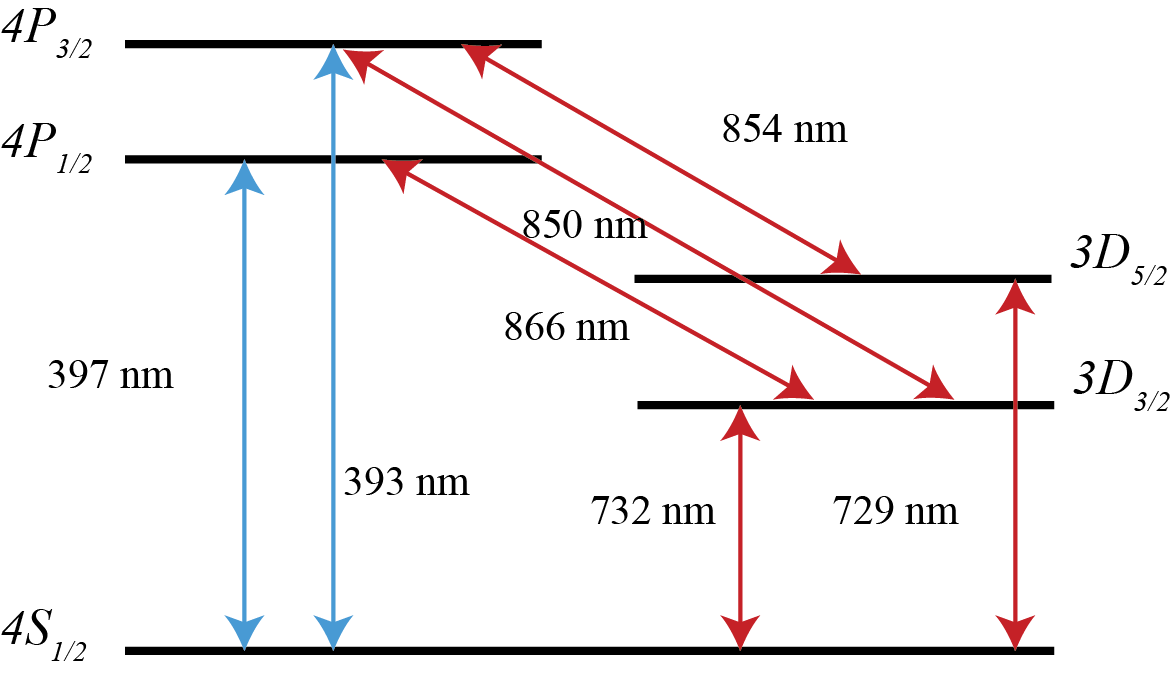
\includegraphics[width=.8\textwidth]{Chapters/Figures/calcium_levels_1-1.PNG}

%\caption will create a figure caption.  Putting an asterisk after it (as in \caption* ) will cause the caption to not be numbered and to not appear in the list of figures.  The [] argument is optional but recommended; this is the short-form caption which will appear in the list of figures.  The {} argument is required, and gives the full caption which will appear in the main text.  The first few words of this caption will be used in the list of figures if no [] form is given.  
\caption[Short-form caption]{Long-form caption that appears in main body of the document}

% the \label gives a reference for this figure so that you can refer to it in the text by its number in a way which will be automatically updated if you change the document.  THIS IS A GOOD IDEA; having automatically updated references for figures, equations, etc, will keep your document in order even as you continue to update it over a period of months.  This reference can be called in the text using the \ref tag.
\label{fig:aFigure}
\end{figure}



Here, back in the main body of the text, we can create a reference to figure \ref{fig:aFigure}.  This is automatic; the actual numbers are not typed into the code, but rather the \texttt{\textbackslash ref} tag has been used.  Always always always use the \texttt{\textbackslash ref} command to reference figures, or invariably at some point you'll move something and all of your references will be incorrect and you'll have to fix them manually.

% Here is the same figure, but now using the wrapfigure environment.  This allows you to wrap your text around the figure itself.  The optional [] argument specifies how many lines of text should be wrapped.  The first {} argument specifies where on the page the figure should live (here the right side is specified).  The second {} argument defines how much real estate on the page will be allocated for the figure block; here it is 45% of the page width.
\begin{wrapfigure}[11]{r}{0.45\textwidth}
\centering
% \vspace creates vertical white space in the document.  Here we are creating 0.1 lines of text worth of negative white space, effectively moving our graphic up in the document by one line.  I find this lines things up better within the text in this case, but you may need to manipulate this to make the alignments look correct.
\vspace{-.1\baselineskip}
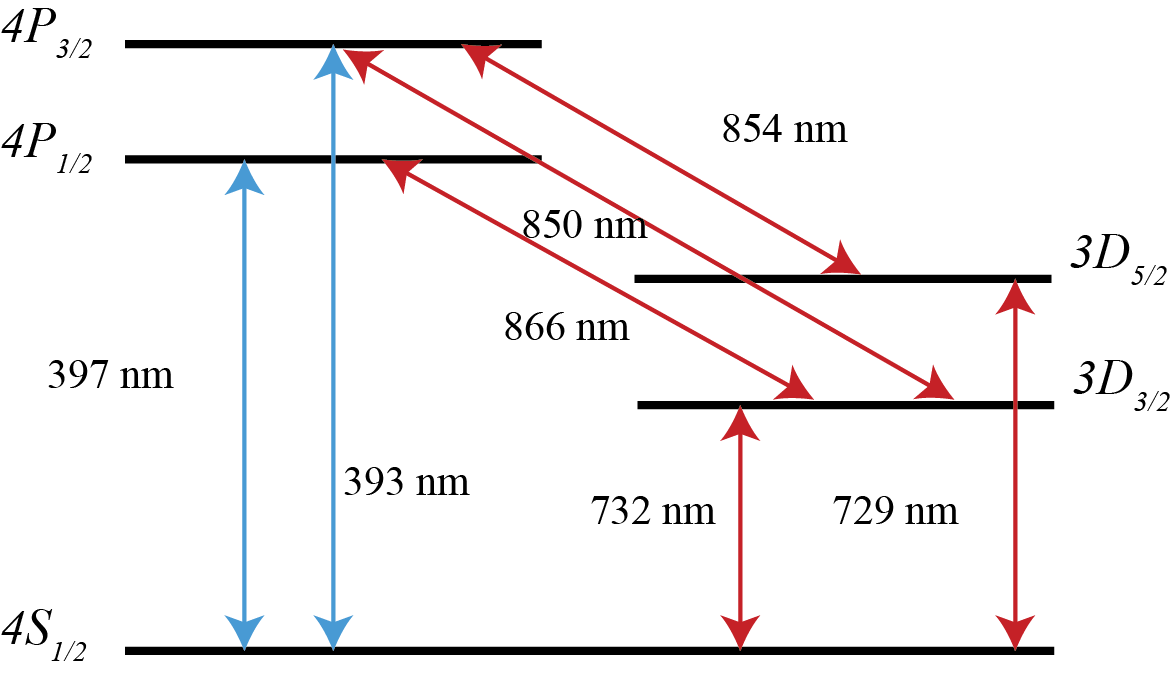
\includegraphics[width=.4\textwidth]{Chapters/Figures/calcium_levels_1-1.PNG}
\caption[Another short-form caption]{A figure included using the wrapfig environment}
\label{fig:anotherFigure}
\end{wrapfigure}
As an alternative to the ordinary figure environment, you might deem it desirable to tuck a figure in more closely amongst the text.  This has a separate environment known as \emph{wrapfig}.  Here we will include the same figure as above a second time, but this time using the \emph{wrapfig} environment.  This will insert the figure into your document with the text wrapping around the perimeter, rather than offsetting it into its own separate chunk of page, as above.    As before, we can use an automated reference to the figure using the \texttt{\textbackslash ref} tag; here we have figure~\ref{fig:anotherFigure}.  Working with the wrapfigure environment sometimes requires a little bit of massaging to ensure that everything lines up properly in your document, but with a small amount of work  you will find that you can get the text to box the figure quite nicely.

Here I have added a table, because tables are also useful. This table has nothing to do with the rest of the material in this thesis template, but you should probably only add relevant tables.
\begin{table}[tbh]
\begin{center}
%\caption[]{\em{Here we show the continuum sensitivity required per band.}}
\begin{tabular}{ccccccc}
\hline \noalign {\smallskip}
Name & SpT & Dist. & Age & 3$\sigma$ M$_{\rm dust}$ & 3$\sigma$ CO(3-2) limit & Disk indicator \\
 & & (pc) & (Myr) & limit (M$_{\oplus}$) &  (mJy km s$^{-1}$)\\
\hline \noalign {\smallskip}
J0226 & L0 & 46.5 & 45 & 0.01 & 24 & Pa$\beta$, IR\\
J0501 & M4.5 & 47.8 & 42 & 0.01 & 23 & H$\alpha$, IR\\
J1546 & M5 & 59.2 & 55 & 0.01 & 14 & HeI, [OI], H$\alpha$, IR\\
J0446 A/B & M6/M6 & 82.6/82.2 & 42 &  0.027 & 18 & H$\alpha$, IR\\
J0949 A/B & M4/M5 & 79.2/78.1 & 45 &  0.024 & 17 & H$\alpha$, IR\\
LDS 5606 A/B & M5/M5 & 84/84 & 30-44 & 0.027 & 19 & H$\alpha$, IR, UV\\
\hline \noalign {\smallskip}
\end{tabular}
\end{center}
\end{table}




\chapter{A second chapter}
% Another mock chapter

Here is a second mock chapter.  As far as the \LaTeX ~is concerned, it is in no way different from the introduction excepting that it appears after it in the main .tex file.  As before, it can be populated with sections, subsections, figures, etc. as you see fit.

In fact, you will probably write perhaps three to six chapters for your thesis depending on how your work is most effectively organized.  Most theses will contain an introduction, at least one `body' chapter, and some sort of conclusions/future directions chapter.  Most theses will also include an appendix or two \ldots


\chapter{Transformers}

\section{Before the Transformers}


The Recurrent Neural Networks or RNN dates from 1986 based on the work of Rumelhart
\cite{Rumelhart}.
The Recurrent Neural Networks or RNN dates from 1986 based on the work of Rumelhart. These networks
are specialized to work with data that contains temporal information and therefore the results
obtained improve against other types such as FeedForward or Convolutional networks.


The main idea behind these models is the concept of Parameter Sharing. Con Parameter Sharing un
modelo puede generalizar mejor cuando la información esta contenida en diferentes partes de una
secuencia. Así el modelo no necesita aprender independientemente todas las reglas que forman la
secuencias, sino que ahora, la salida para cada elemento en el tiempo esta determinada por la
salida del elemento anterior. Resultando en una recurrencia con las mismas reglas de actualización
aplicadas a cada elemento en el tiempo.

y visto como un gráfo computacional dirigído y acíclico.

\begin{equation}
    s^{(t)} = f(s^{(t-1)}; \theta)
\end{equation}


% the \appendix tag tells LaTeX where it should start labeling chapters with letters (denoting appendices) rather than numbers (denoting main chapters)
\appendix


\chapter{An appendix}
% Look!  An Appendix!

% Appendices are a good idea for almost any thesis.  Your main thesis body will likely contain perhaps 40-60 pages of text and figures.  You may well write a larger document than this, but chances are that some of the information contained therein, while important, does \emph{not} merit a place in the main body of the document.  This sort of content - peripheral clarifying details, computer code, information of use to future students but not critical to understanding your work \ldots - should be allocated to one or several appendices.




% \bibliographystyle tells LaTeX how you want to format your bibliography.  There are many standard formats.  apsrev is fairly typical, but feel free to explore other options if the mood strikes.
\bibliographystyle{ieeetr}

% \bibliography calls the actual file that contains your bibliographic information.  This file can be generated by hand or in an automated way using software such as BibTeX.  Either works fine, but it is worth learning to use BibTex in the long term.  Take a look at the .bib file included here if you want to get some idea of the formatting required to create a bibliogrphy file of your own.

\bibliography{bibliography}
\end{document}
